\section{Experiment}

The main goal of experiments is to test the denoising ability of the MeanFlow framework. We hope to verify that the MeanFlow model can generate clean images from noisy images with only a single function evaluation.

%%%%%%%%%%%%%%%%%%%%%%%%%%%%%%%%%%%%%%%%%%
% Experiment Setup
%%%%%%%%%%%%%%%%%%%%%%%%%%%%%%%%%%%%%%%%%%
\subsection{Experiment Setup}

{
\setlength{\parindent}{0pt}

\textbf{Dataset.} We conduct experiments on the MNIST dataset. Noisy inputs (from $p_\text{prior}$) are generated by adding Gaussian noise to the original clean images: $\text{noisy-img} = \text{clean-img} + \sigma \epsilon$, where $\epsilon$ is a standard Gaussian noise and $\sigma$ is a random variable uniformly distributed in $\text{Uniform}(0.3, 0.8)$. We choose this range for $\sigma$ because when $\sigma > 1$, the noisy input becomes almost unrecognizable and resembles pure Gaussian noise, and when $\sigma < 0.2$, the images remain clear, leaving little need for denoising.

\vspace{1em}

\textbf{Model Configuration.}
We adopt the DiT structure described in Section~\ref{sec:dit} to parameterize the average velocity field. In this experiment, the model is set with an input size of $(1 \times 32 \times32)$, a patch size of $(2 \times 2)$, an embedding dimension $d=144$, $6$ DiT blocks, and $3$ attention heads per block. Time and label information are combined via a lightweight MLP and added to each transformer block using adaptive LayerNorm (adaLN).

\vspace{1em}

\textbf{Loss Metric.}
We adopt the adaptive L2 loss following~\cite{meanflow}. For a regression error $\Delta$, the loss is computed with:
$L = \text{sg}[w] \cdot \|\Delta\|_2^2$, where $w = \dfrac{1}{(\|\Delta\|_2^2 + c)^p}$ and $p = 1-\gamma$. In our experiments, we set $\gamma=0.5$ and $c=10^{-3}$. This setting down-weights large errors and stabilizes training.

\vspace{1em}

\textbf{Sampling $(r, t)$.}
For each training step, time indices $(r, t)$ are sampled from a logit-normal distribution following~\cite{meanflow}. Specifically, we draw two samples from $\mathcal{N}(\mu,\sigma)$ (with $\mu=-0.4$, $\sigma=1.0$), and pass them through a logistic sigmoid to map them into $(0,1)$. Then the larger one is assigned to $t$, and the smaller one is assigned to $r$. We set a certain portion of random samples with $t = r$.

\vspace{1em}

\textbf{Training Details.}
The model is optimized using AdamW with an initial learning rate of $1\times 10^{-4}$, no weight decay, and a batch size of 128, for a total of $300k$ update steps.
%
The learning rate is scheduled by cosine annealing with warm restarts. The initial period is $10k$ steps and doubles after each restart, with a lower bound of $1 \times 10^{-6}$.
%
Mixed-precision training (FP16) is employed through \texttt{accelerate.Accelerator} to reduce memory consumption and improve efficiency.
%
During training, intermediate checkpoints, denoised samples, and the denoising performance (PSNR) are regularly saved.
}

%%%%%%%%%%%%%%%%%%%%%%%%%%%%%%%%%%%%%%%%%%
% 伪代码和流程图
%%%%%%%%%%%%%%%%%%%%%%%%%%%%%%%%%%%%%%%%%%
\begin{minipage}[t]{0.48\textwidth}
  \vspace{0pt} % 强制顶部对齐
  \RestyleAlgo{ruled}
  \begin{algorithm}[H]
      \caption{Training MeanFlow DiT}\label{alg:training}
  \ForEach{$\text{Batch of } (x_0, z) \in \text{Dataset}$}{
    sample $(r, t)$ \;
    compute $x_r = (1-r) x_0 + r z$ \;
    compute $v(x_r, r \mid z) = z - x_0$ \;
    compute $u, {d u}/{d r}$ with \texttt{jvp} \;
    $u^\text{tgt} = v - (t - r) \frac{d u}{d r}$ \;
    error $e = u - \text{sg}[u^\text{tgt}]$ \;
    compute loss $\mathcal{L}(\theta)$ \;
    update $\theta$ \;
  }
  \end{algorithm}
\end{minipage}%
\hfill
\begin{minipage}[t]{0.48\textwidth}
  \vspace{0pt} % 强制顶部对齐
  \centering
  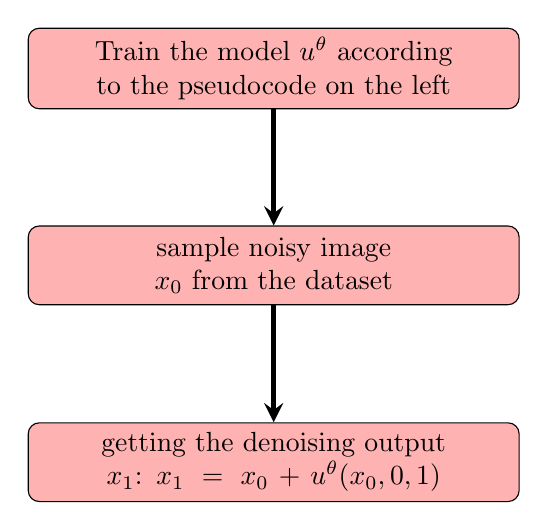
\begin{tikzpicture}[node distance=2.5cm]
    \tikzstyle{rednode} = [rectangle, rounded corners,
      minimum width=6cm, minimum height=1cm, text width=6cm, align=center,
      draw=black, fill=red!30]
    \tikzstyle{arrow} = [thick,->,>=stealth, line width=2pt]

    \node (step1) [rednode] {Train the model $u^\theta$ according to the pseudocode on the left};
    \node (step2) [rednode, below of=step1] {sample noisy image $x_0$ from the dataset};
    \node (step3) [rednode, below of=step2] {getting the denoising output $x_1$: $x_1 = x_0 + u^\theta(x_0, 0, 1)$};

    \draw [arrow] (step1) -- (step2);
    \draw [arrow] (step2) -- (step3);
  \end{tikzpicture}
  \captionof{figure}{Total Pipeline}\label{fig:pipeline}
\end{minipage}


%%%%%%%%%%%%%%%%%%%%%%%%%%%%%%%%%%%%%%%%%%
% Results and Analysis
%%%%%%%%%%%%%%%%%%%%%%%%%%%%%%%%%%%%%%%%%%
\subsection{Results and Analysis}

Our MeanFlow denoising model is evaluated on the MNIST dataset. Figure~\ref{psnr_over_step} shows the PSNR values of 1-NFE denoising result during training, indicating that the model consistently improves as the number of update steps increases. The learning rate and loss during training are provided in Appendix~\ref{app:rate_and_loss}.

Table~\ref{tab:psnr_over_step} summarizes PSNR values at different training stages, confirming steady enhancement of denoising quality over time. Table~\ref{tab:psnr_over_nfe} presents the denoising performance after 300k training steps under different numbers of function evaluations (NFE). Increasing NFE from 1 to 2 yields significant gains, while further increases produce little improvements. This suggests a performance saturation at higher NFEs.

\vspace{1cm}
\begin{minipage}[c]{\linewidth}
  \centering
  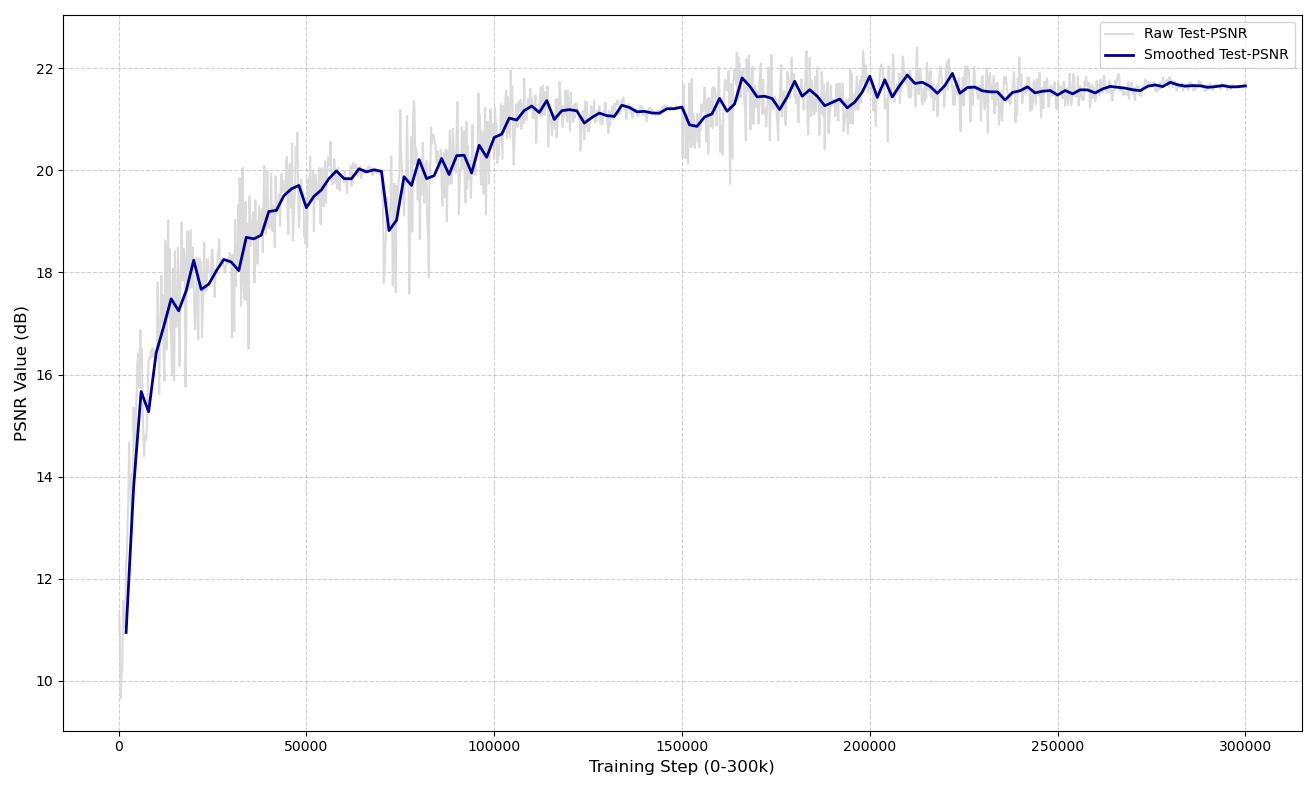
\includegraphics[width=0.8\linewidth]{figures/psnr_over_step.png}
  \captionof{figure}{PSNR values over training steps for 1-NFE denoising.}\label{psnr_over_step}
\end{minipage}
\vspace{1cm}

\begin{minipage}[c]{0.48\linewidth}
  \centering
  \begin{tabular}{cc}
    \toprule
    \textbf{Training Step} & \textbf{PSNR (dB)} \\
    \midrule
    Noisy Input & 5.9312 \\
    2k & 12.3043 \\
    20k & 17.7944 \\
    100k & 20.2236 \\
    200k & 21.6694 \\
    300k & 21.6807 \\
    \bottomrule
  \end{tabular}
  \captionof{table}{PSNR over training steps.}\label{tab:psnr_over_step}
\end{minipage}
\hfill
\begin{minipage}[c]{0.48\linewidth}
  \centering
  \begin{tabular}{cc}
    \toprule
    \textbf{NFE} & \textbf{PSNR (dB)} \\
    \midrule
    Noisy Input & 6.0401 \\
    1 & 22.6455 \\
    2 & 24.0686 \\
    3 & 24.0816 \\
    4 & 24.0691 \\
    5 & 24.0558 \\
    \bottomrule
  \end{tabular}
  \captionof{table}{Denoising performance under different NFE.}\label{tab:psnr_over_nfe}
\end{minipage}
\vspace{1cm}

Visual comparison of denoising results under different NFEs are provided in Figure~\ref{fig:mnist_img}. The top row shows the ground truth images, followed by the noisy inputs, and denoised outputs after 1 to 5 NFEs. It's observed that even a single NFE produces notable noise reduction.

\begin{minipage}[c]{\linewidth}
    \centering
    % Visual results
    \noindent
    \begin{minipage}[c]{0.92\linewidth}
        
\includegraphics[width=\linewidth]{figures/mnist_img/clean.png}%
    \end{minipage}%
    \begin{minipage}[c]{0.07\linewidth}
        \centering
        {\small GT}
    \end{minipage}

    \noindent
    \begin{minipage}[c]{0.92\linewidth}
        
\includegraphics[width=\linewidth]{figures/mnist_img/noised.png}%
    \end{minipage}%
    \begin{minipage}[c]{0.07\linewidth}
        \centering
        {\small Input}
    \end{minipage}

    \noindent
    \begin{minipage}[c]{0.92\linewidth}
        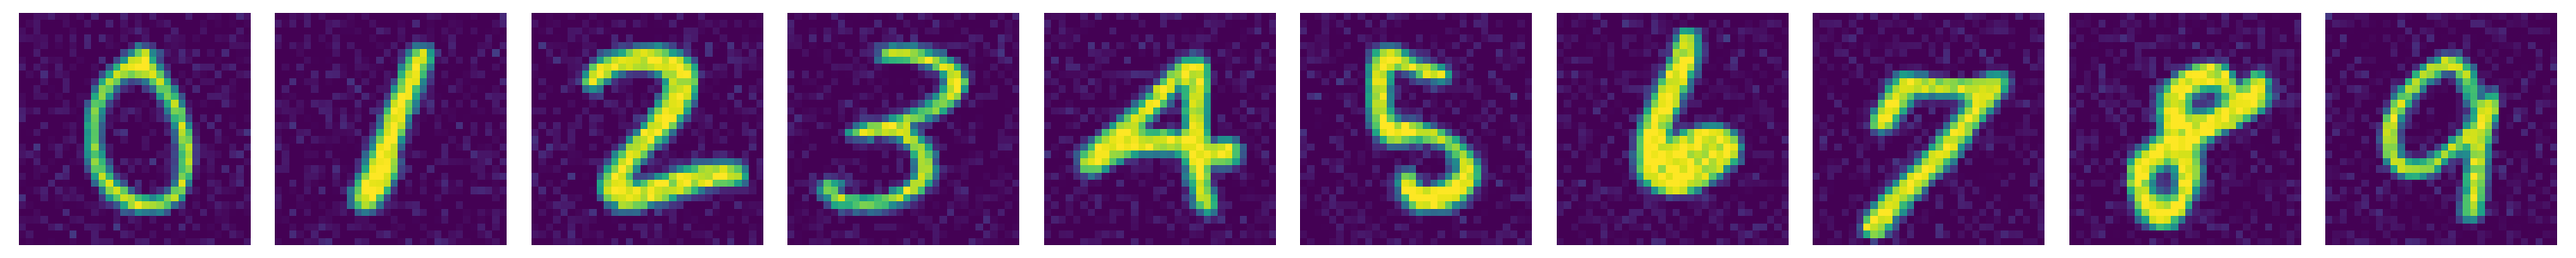
\includegraphics[width=\linewidth]{figures/mnist_img/nfe_1.png}%
    \end{minipage}%
    \begin{minipage}[c]{0.07\linewidth}
        \centering
        {\small 1-NFE}
    \end{minipage}

    \noindent
    \begin{minipage}[c]{0.92\linewidth}
      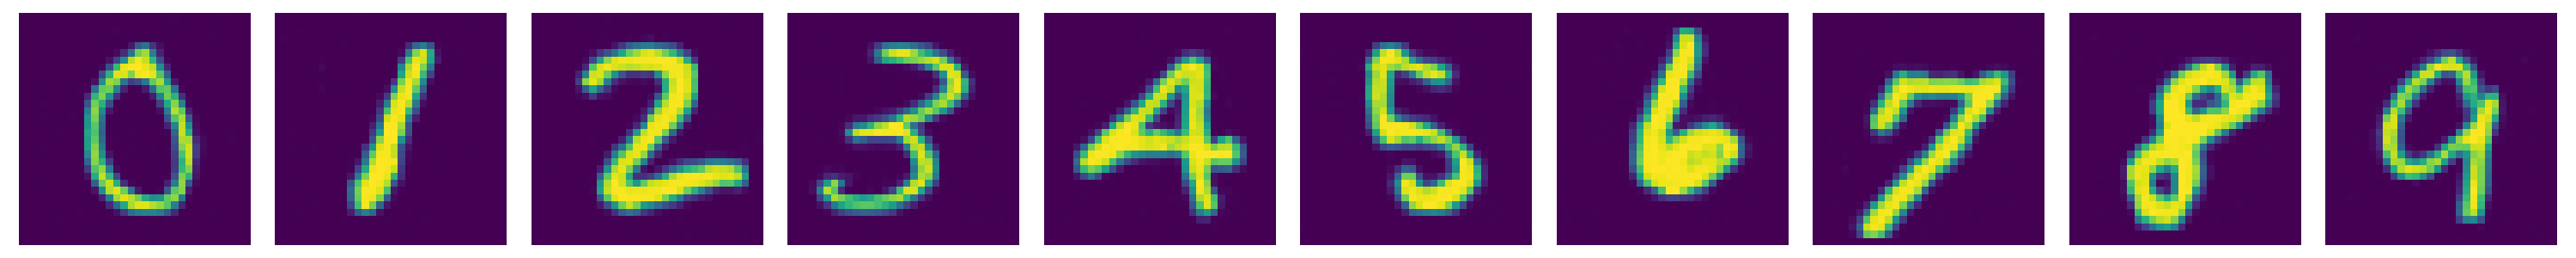
\includegraphics[width=\linewidth]{figures/mnist_img/nfe_2.png}%
    \end{minipage}
    \begin{minipage}[c]{0.07\linewidth}
      \centering
      {\small 2-NFE}
    \end{minipage}

    \noindent
    \begin{minipage}[c]{0.92\linewidth}
      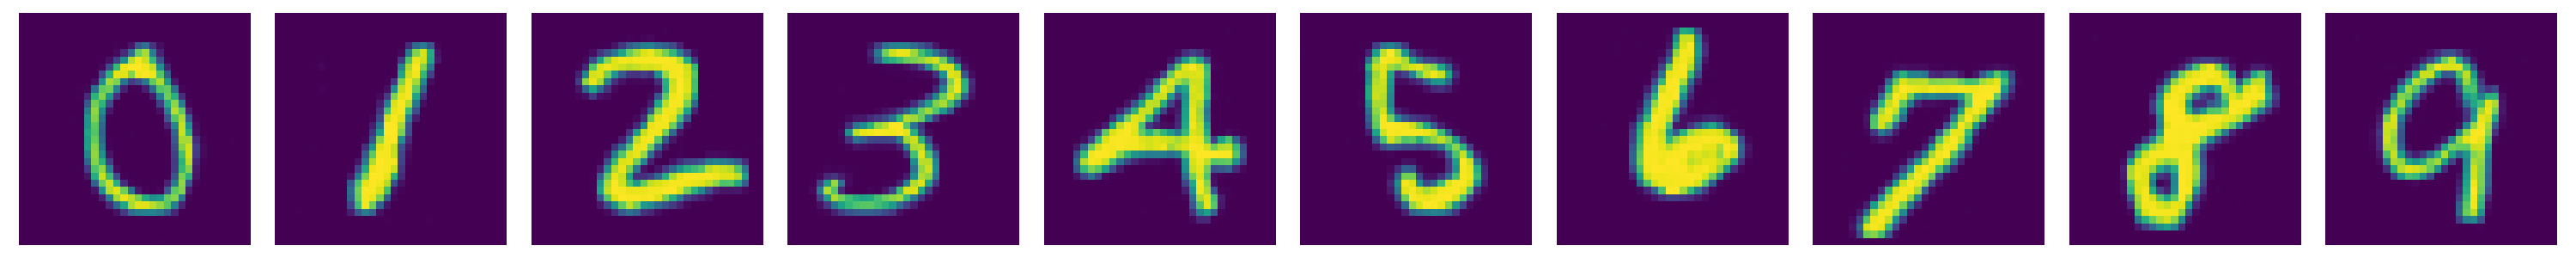
\includegraphics[width=\linewidth]{figures/mnist_img/nfe_3.png}
    \end{minipage}
    \begin{minipage}[c]{0.07\linewidth}
      \centering
      {\small 3-NFE}
    \end{minipage}

    \noindent
    \begin{minipage}[c]{0.92\linewidth}
      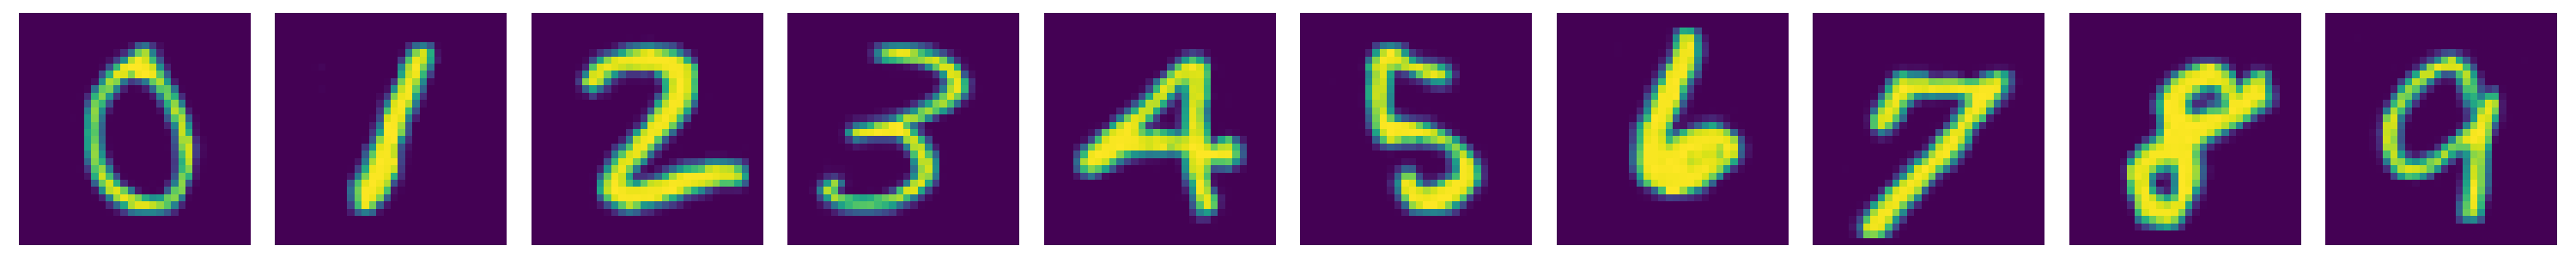
\includegraphics[width=\linewidth]{figures/mnist_img/nfe_4.png}
    \end{minipage}
    \begin{minipage}[c]{0.07\linewidth}
      \centering
      {\small 4-NFE}
    \end{minipage}

    \noindent
    \begin{minipage}[c]{0.92\linewidth}
      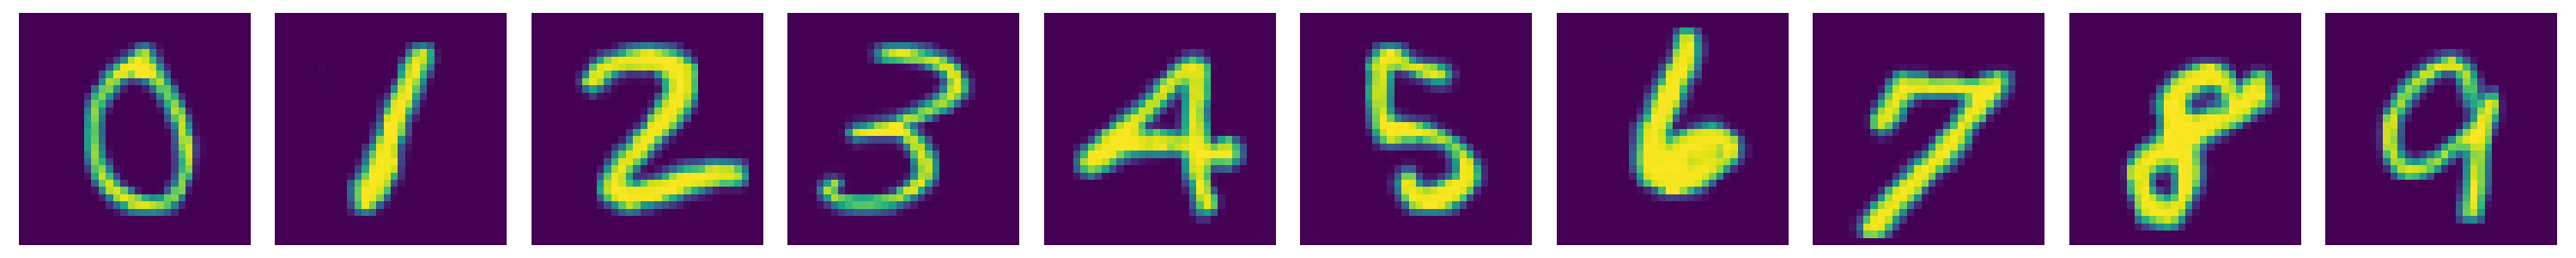
\includegraphics[width=\linewidth]{figures/mnist_img/nfe_5.png}
    \end{minipage}
    \begin{minipage}[c]{0.07\linewidth}
      \centering
      {\small 5-NFE}
    \end{minipage}

    \captionof{figure}{Visual comparison of denoising results under different NFEs. From top to bottom: ground truth, noisy input, and model outputs after 1 to 5 NFE steps.}\label{fig:mnist_img}
\end{minipage}
